
\documentclass[a4paper]{article}
\usepackage[left=3cm,right=3cm,top=2cm,bottom=2cm]{geometry} % page settings
\usepackage{amsmath} % provides many mathematical environments & tools
\usepackage{titlesec}
\usepackage{graphicx}
\usepackage{algorithm,caption}
\usepackage[utf8]{inputenc}
\usepackage[noend]{algpseudocode}
\graphicspath{ {images/} }
\usepackage{xparse}% http://ctan.org/pkg/xparse
\usepackage{mathtools}
\usepackage{courier}
\usepackage{verbatim}
\DeclarePairedDelimiter\ceil{\lceil}{\rceil}
\DeclarePairedDelimiter\floor{\lfloor}{\rfloor}


\setlength{\parindent}{0mm}
\titleformat{\subsection}[runin]
{\normalfont\Large\bfseries}{\thesection}{1em}{}
\titleformat{\subsubsection}[runin]
{\normalfont\large\bfseries}{\thesubsection}{1em}{}

\begin{document}
	
	\title{Secure \& Dependable Systems \\  Spring 2017 \\ Assignment 04}
	\author{Humza Abid}
	\maketitle
	
	\subsection*{Problem 4.1} \textit{Verification}: \\
	
	\textbf{Factorial:}
	
	\begin{figure}[ht]
		\centering
		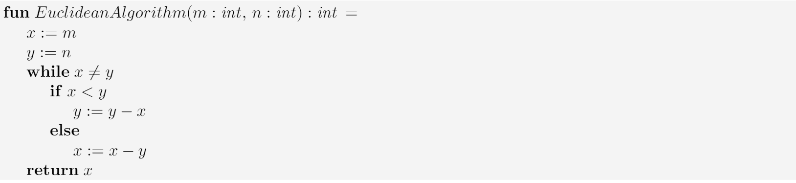
\includegraphics[width=0.7\textwidth, scale=0.7]{euc_snippet.png}
		\caption*{}
		\label{euc}
	\end{figure}
	
	Precondition:
		
	\begin{verbatim}
		P(n) := n > 0
	\end{verbatim}
	
	Postcondition:
	
	\begin{verbatim}
	Q (n, product) := n! == product 
	\end{verbatim}
		
	Loop invariant:
	
	\begin{verbatim}
		I := product == (factor-1)!    
	\end{verbatim}
	
	Partial Correctness (Somewhat informal):\\
	
	This algorithm is correct because the loop invariant will always be true since $n!$ is defined as $n*(n-1)!$ It will always terminate because factor starts at 1 and increases by one each time round the loop, the factor must therefore reach n. \\
	
	
	\textbf{Euclidean:}

	\begin{figure}[ht]
		\centering
		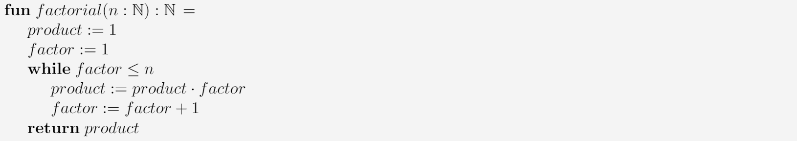
\includegraphics[width=0.7\textwidth, scale=0.7]{factorial_snippet.png}
		\caption*{}
		\label{factorial}
	\end{figure}
	
	Precondition:
	
	\begin{verbatim}
		P(m, n) := m > 0 , n > 0
	\end{verbatim}
	
	Postcondition:
	
	\begin{verbatim}
		Q (m, n, x) := x == GCD(m, n)
	\end{verbatim}
	
	\pagebreak
	
	Loop invariant:
	
	\begin{verbatim}
		I = GCD(x, y) == GCD(m, n)        
	\end{verbatim}
	
	Partial Correctness: \\
	
	Base Case:  When the code first reaches the loop test, x is still equal to m, and y is still equal to n, so the loop invariant trivially holds. \\
	
	Induction:  Assume that the loop invariant holds at the loop test, and also that the loop test passes.
	Let $x_f$ and $y_f$ be the values of m and n at the bottom of the loop.  Consider two cases.  If $(x < y)$, then $y_f = y - x$, $y_f$ is positive, and $GCD(x, y_f) = GCD(x, y)$, because any
	number that divides x and y also divides $y - x$.  The other case is similar, except that $x_f$ might be 0.  In both cases, $GCD(x_f, y_f) = GCD(m, n) = GCD(m, n)$, and $x_f \ge 0$,
	and $y_f \ge 0$, so the loop invariant holds.\textbf{QED}.
	
	\subsection*{Problem 4.2} \textit{Dynamic Logic: Practice}: \\
	
	I downloaded the latest binary build for KeY on my system. I loaded a built in Java function, SumAndMax function. The function, as the name suggests, computes and returns the sum and the maximum of a given n element array. The pre and post conditions are presented below.
	
	\begin{figure}[ht]
		\centering
		
\includegraphics[width=1\textwidth, scale=0.7]{prepost.png}
		\caption*{}
		\label{prepost}
	\end{figure}	
	
	The following succession of snapshots is walks us through the program, the displaying the code used, the proof tree and a summary of the process. 
	
	\begin{figure}[h!]
		\centering
		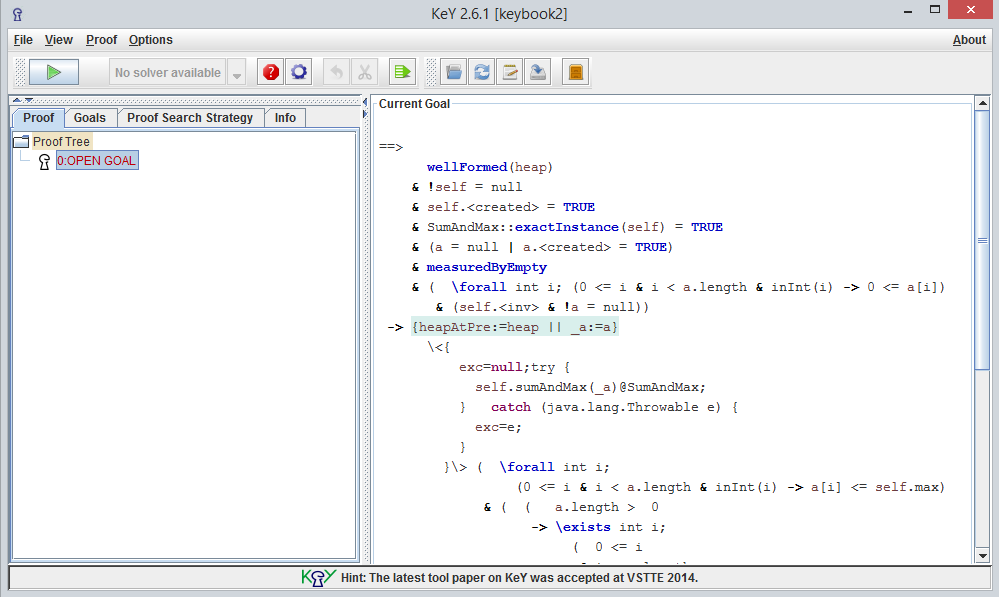
\includegraphics[width=0.7\textwidth, scale=0.7]{421.png}
		\caption*{}
		\label{1}
	\end{figure}	
	
	\begin{figure}[h!]
		\centering
		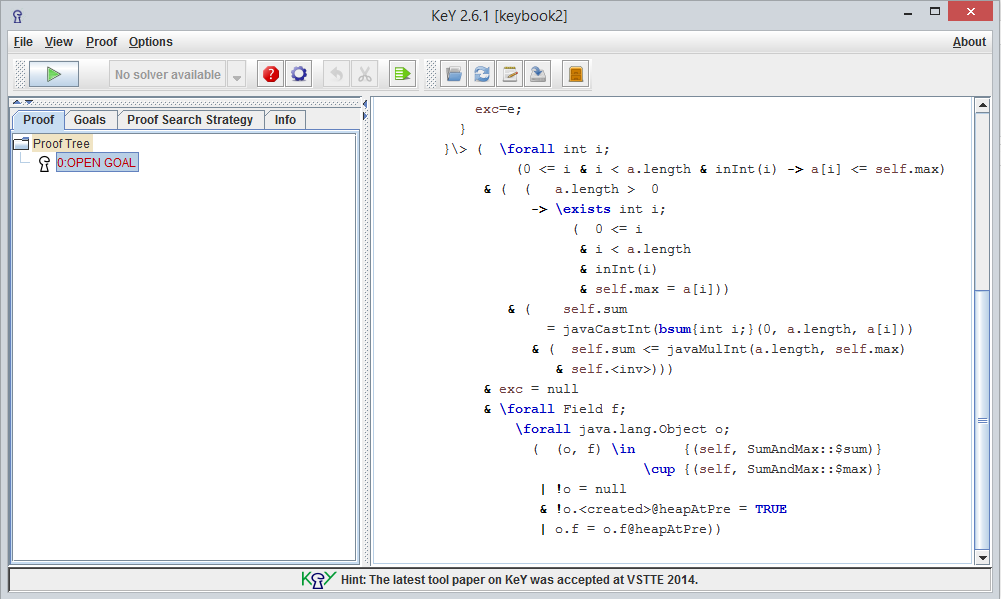
\includegraphics[width=0.7\textwidth, scale=0.7]{422.png}
		\caption*{}
		\label{2}
	\end{figure}
	
	\begin{figure}[h!]
		\centering
		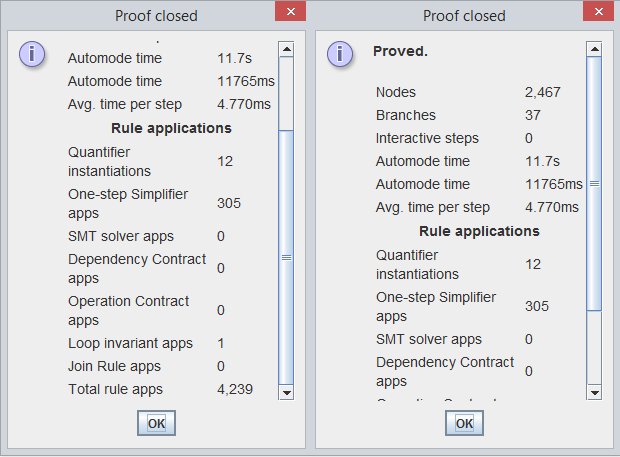
\includegraphics[width=0.5\textwidth, scale=0.05]{424.png}
		\caption*{}
		\label{3}
	\end{figure}	

	\begin{figure}[h!]
		\centering
		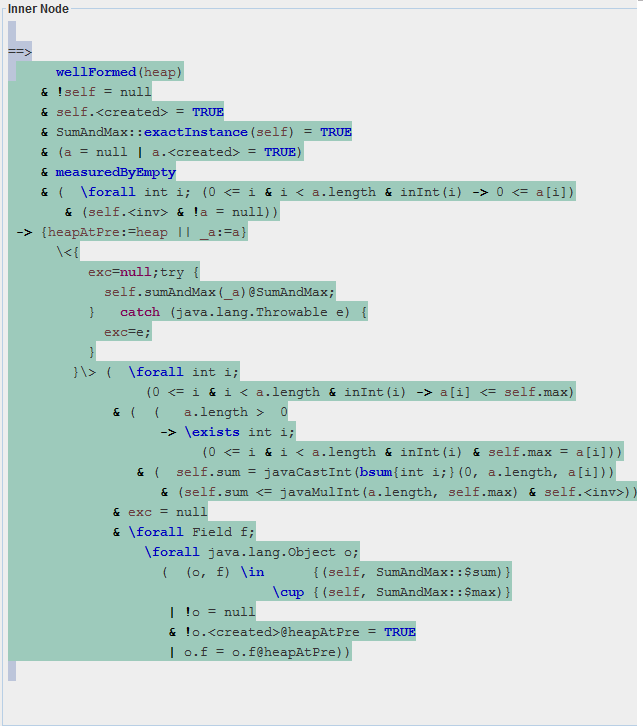
\includegraphics[width=0.5\textwidth, scale=0.7]{425.png}
		\caption*{}
		\label{4}
	\end{figure}
	
	
	\newpage
	\subsection*{Problem 4.3} \textit{Soundness}: \\
	
	
	\textbf{while:} \\
	
	\texttt{while} $\phi [\delta]$ \texttt{do} $\delta \coloneqq R[\delta]$ \\
	
	Here, $l[\delta]$ is the loop invariant, $\phi[\delta]$ and $R[\delta]$ are the loop condition and function representing the update of the variable $\delta$ performed in the loop body, respectively.\\ 
	
	\begin{equation}
		\forall_{\delta \colon l[\delta]} f[\delta] = 
			\begin{cases} 
				\hfill \delta    \hfill & \text{ if $\neg \phi [\delta]$} \\
				\hfill f[R[\delta]] \hfill & \text{ if $\phi [\delta]$} \\
			\end{cases}
	\end{equation}
	
	\begin{equation}
		\forall_{\delta \colon l[\delta]} l[R[\delta]]
	\end{equation}
	
	\begin{equation}
		\forall_{\delta \colon l[\delta]} \wedge 
		\left \{
		\begin{tabular}{c}
		$\neg \phi [\delta] \implies \pi [\delta]$\\
		$\phi [\delta] \wedge \pi [R[\delta]] \implies \pi [\delta]$\\
		\end{tabular}
		\right \} \implies \forall_{\delta \colon l[\delta]} pi[\delta]
	\end{equation}
	
	and finally:
	
	\begin{equation}
	\forall_{\delta \colon l[\delta]} l[f[\delta]]
	\end{equation} \\
	
	To summarize: (4) follows from the semantics (1) and the termination condition (3). \\
	
	\textbf{if:} \\
	
	\[\frac{\{B \wedge P\} S\{Q\} \text{ , } \{\neg B \wedge P\} T\{Q\}}{\{P\} \text{ if } B \text{ then } S \text{ else } T \text{ endif } \{Q\}}\] \\
	
	A postcondition Q common to the then and else part is also a postcondition of the whole if...endif statement. In the then and the else part, the unnegated and negated condition B can be added to the precondition P, respectively. The condition, B, must not have side effects. \\
	
	if \texttt{B} then \texttt{S} else \texttt{T} endif is equivalent to :\\
	
	bool b $\coloneqq$ true; while \texttt{B} $\wedge$ \texttt{b}  do \texttt{S}; \texttt{b} $\coloneqq$ false done; \texttt{b} $\coloneqq$ true; while $\neg$ \texttt{B} $\wedge$ \texttt{b} do \texttt{T}; b $\coloneqq$ false done.
	
	
	 
\end{document}